%!TEX root = thesis.tex
\subsection{Größe} % (fold)
\label{sub:gr_e}
Die Testreihe, um die Auswirkung der Größe (in Knoten) eines Graphen auf die Algorithmen zu erforschen, orientiert sich an einem Socialgraph. Es wurde geschätzt, dass jede Person eines Social Networks durchschnittlich 100 Freunde hat, dass jeder mehr als einen und keiner mehr als 500 Freunde hat. Auf die Maßzahlen eines Graphen übetragen, bedeutet das, dass alle Graphen dieser Testreihe einen durchschnittlichen Knotengrad von 100 haben, wobei der Knotengrad immer zwischen 1 und 500 liegt. Variiert wurde nun die Größe der Graphen, also die Anzahl der Knoten. Verglichen mit den anderen beiden Testreihen handelt es sich hier um relativ dünn besetzte Graphen, so dass selbst der größte verwendete Graph mit 500 000 Knoten noch unter 500 MB liegt. Es wurde versucht, die Graphgröße weiter auf bis zu 2 Millionen Knoten zu steigern, was allerdings nicht möglich war. Graphen mit vielen Knoten resultieren in großen Sendepuffern und wie sich herausstellte, ist X10 dem nicht gewachsen. Der Sendevorgang (der \textit{at} Block) blockiert das Programm in den meisten Fällen endlos. Deswegen wurde hier die Knotenzahl auf \nobreak{500 000} beschränkt. Es ist zu vermuten, dass diese Größe nicht ausreicht, um gute Ergebnisse bei der Parallelisierung zu erreichen.

Des Weiteren wurde in dieser Testreihe der Modus mit 9 Places und der invasive Algorithmus weggelassen. Dass mit 9 Places auf 8 Kernen die Performance nicht gut sein würde, war zu erwarten und bestätigte sich in den anderen Testreihen. Dass der invasive Algorithmus weggelassen wurde, liegt daran, dass er ebenso Probleme mit der Graphengröße hatte, was zwar durch Implementierungstricks umgangen werden könnte, aber allerdings den Zeitrahmen gesprengt hätte. Wieso genau der invasive Algorithmus nicht funktioniert, ist unten in der Bemerkung erläutert.

Bei jedem Graphen dieser Testreihe war die serielle Version am schnellsten, was nach den vorangegangenen Ergebnissen nicht zu erwarten war. Die serielle Version war schneller als jeder andere Algorithmus, egal mit wie vielen Places. Im Kapitel \ref{sub:dichte}, in dem die Dichte variierte, war der 1D-Algorithmus im Fall mit nur einem Place schneller, als der serielle Algorithmus. Da das in dieser Testreihe nicht so ist, ist zu vermuten, dass der 1D Algorithmus für dichte Graphen ein wenig schneller zu sein scheint, während der serielle Algorithmus für dünn besetzte Graphen schneller ist.

Vergleicht man nur den 1D-Algorithmus mit sich selbst bei steigender Anzahl an Places, zeichnet sich ab, dass 2 Places das Maximum an Parallelität zu sein scheint, dass sich noch lohnt. In Abbildung \ref{fig:groesse_speedup} ist gut zu erkennen, dass der Algorithmus mit 2 Places immer schneller war, als der Algorithmus mit 4 Places. Bei 8 Places war der Speedup immer kleiner als 1, was eine langsamere Laufzeit als die Referenzzeit bedeutet. Wie zu erwarten, steigt tendenziell mit der Anzahl der Knoten das Parallelisierungspotential, wobei es durch den dünn besetzte Graph einigermaßen beschränkt zu sein scheint. Wäre dem nicht so, müsste bei steigender Knotenzahl der Algorithmus mit 4 Places gegenüber den 2 Places aufholen.

Für den 2D Algorithmus gilt, dass nie ein Speedup größer als 1 erreicht wurde. Die hier verwendeten Graphen sind dafür zu klein.

\begin{figure}
	\centering
	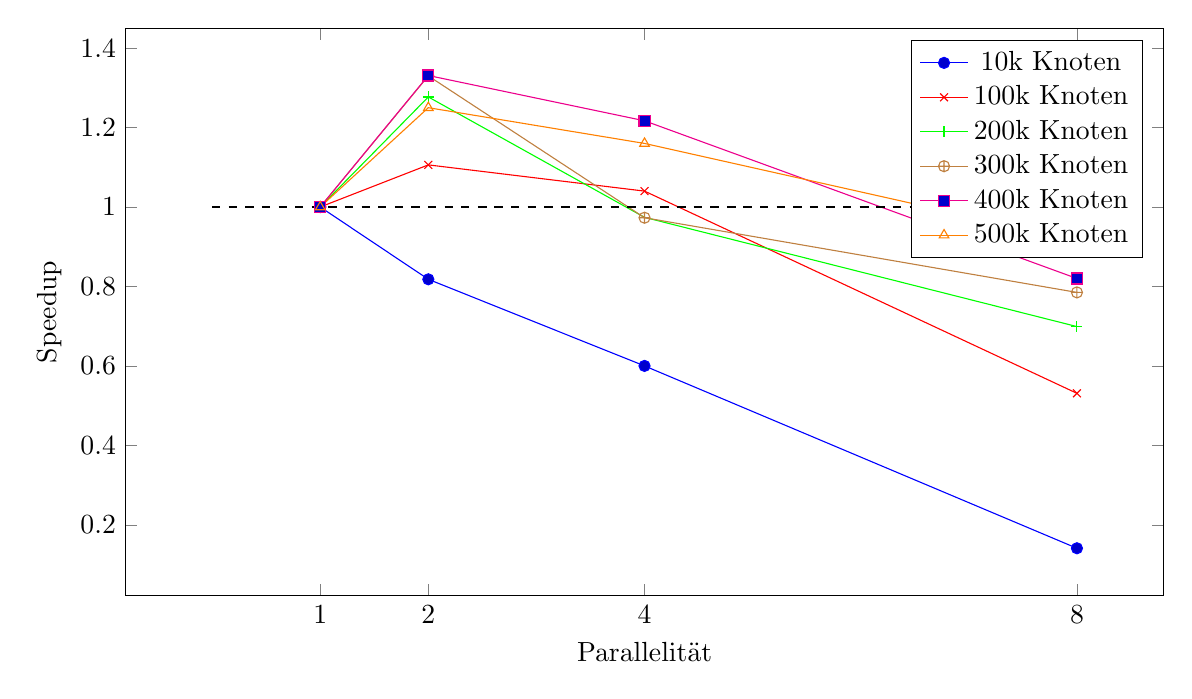
\begin{tikzpicture}
		\begin{axis}[
	        xtick={1,2,4,8},
	        xlabel=Parallelität,
	        ylabel=Speedup,
	        width=420, height=250]

		    \addplot+[
		    blue,
		    solid,
		    mark=*]
		    coordinates {
		        (1,1)
		        (2,0.818)
		        (4,0.6)
		        (8,0.141)
		    };
		    \addlegendentry{10k Knoten}

		    \addplot+[
		    red,
		    solid,
		    mark=x]
		    coordinates {
		        (1,1)
		        (2,1.106)
		        (4,1.04)
		        (8,0.531)
		    };
		    \addlegendentry{100k Knoten}

		    \addplot+[
		    green,
		    solid,
		    mark=+]
		    coordinates {
		        (1,1)
		        (2,1.277)
		        (4,0.974)
		        (8,0.699)
		    };
		    \addlegendentry{200k Knoten}

		    \addplot+[
		    brown,
		    solid,
		    mark=oplus]
		    coordinates {
		        (1,1)
		        (2,1.330)
		        (4,0.973)
		        (8,0.785)
		    };
		    \addlegendentry{300k Knoten}

		    \addplot+[
		    magenta,
		    solid,
		    mark=square*]
		    coordinates {
		        (1,1)
		        (2,1.331)
		        (4,1.217)
		        (8,0.82)
		    };
		    \addlegendentry{400k Knoten}

		    \addplot+[
		    orange,
		    solid,
		    mark=triangle]
		    coordinates {
		        (1,1)
		        (2,1.25)
		        (4,1.16)
		        (8,0.916)
		    };
		    \addlegendentry{500k Knoten}

		    \addplot+[
		        smooth,
		        dashed,
		        black,
		        mark=none]
		    coordinates {
		    	(0,1)
		    	(8,1)
		    };

		\end{axis}
	\end{tikzpicture}
	\caption{Speedup des 1D-Algorithmus über Anzahl der Places. Variiert wurde die Größe des Graphen. Als Referenzwert wurde jeweils der 1D-Algorithmus mit einem Place genommen. Eine Kurve pro Graph.}
	\label{fig:groesse_speedup}
\end{figure}

\underline{Bemerkung:}
Beim Parsen der Graphdatei gehen alle Implementierungen so vor, dass sie Zeile für Zeile in die Datenstruktur eingepflegt werden. Dabei steht schon vor dem Parsen fest, welches Datum später auf welchem Place liegen muss. Die Informationshäppchen, die von Place zu Place übertragen werden müssen, sind relativ klein. Im invasiven Fall ergibt es wenig Sinn, schon ein \textit{invade} aufzurufen, bevor überhaupt der Graph eingelesen wurde, bevor also die Größe des Problems bekannt ist. Aus diesem Grund wird der Graph erst lokal auf den ersten Place eingelesen, dann der Constraint zusammengebaut und erst wenn der Claim bekannt ist, auf die involvierten Places verteilt. Die hier zu übertragenen Daten sind relativ groß, womit X10 Probleme zu haben scheint. Das Problem könnte umgangen werden, indem die Datenstruktur in kleinere Häppchen aufgeteilt wird. Das ist aber höchstens ein Workaround für ein Problem, das bei X10 liegt.
% subsection gr_e (end)